\chapter{Data Structures}
\label{chap:appendixds}

%##################################################################################################
\section{Disjoint Set Forests}
\label{sec:appendixds-dsf}
%##################################################################################################

\index{disjoint set forests|(}

Echoing the more general definition of partitioning in Chapter~\ref{chap:ipfs}, we first observe that:

\begin{definition}
A set of k subsets $\{S'_1,\ldots,S'_k\}$ \textbf{partitions} a set $S$ iff:

\begin{enumerate}
\item $\bigcup_i S'_i = S$ and
\item $\forall i,j \cdot i \ne j \Rightarrow S'_i \cap S'_j = \emptyset$.
\end{enumerate}

\noindent (In words, the subsets together make up $S$, and are mutually disjoint.)
\end{definition}

\noindent \textbf{Disjoint set forests} (DSFs), which are a staple of undergraduate computer science courses \cite{worrell06}, are a data structure designed to represent such a partition using a collection of trees, one for each subset (see Figure~\ref{fig:appendixds-dsf-representation}). Each subset has a \emph{representative element}, namely the root node of its tree. The goal is to efficiently support three key operations:

%---
\stufigex{height=3.5cm}{appendixds/appendixds-dsf-representation.png}{An example disjoint set forest, representing the partitioning of the set $\{A \ldots L\}$ into disjoint subsets $\{A,B,C,E\}$, $\{D,F,G,H,I\}$, $\{K,L\}$ and $\{J\}$}{fig:appendixds-dsf-representation}{p}
%---

\begin{enumerate}

\item MAKE-SET, which makes a subset containing a single element.
\item FIND-SET, which allows the lookup of the representative element of the subset containing a particular element.
\item UNION, which allows the (distinct) subsets containing two individual elements to be merged.

\end{enumerate}
%
The basic idea (initially ignoring the details) is that MAKE-SET makes a single node tree, FIND-SET follows the path from a given element to the top of its tree and returns the root, and UNION merges trees by making the root of one the child of the root of the other (see Figure~\ref{fig:appendixds-dsf-unionexample}). However, in order to make things more efficient, two optimizations are commonly employed:

%---
\begin{stusubfig}{p}
	\subfigure[The initial forest]
	{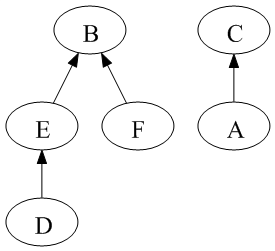
\includegraphics[height=3.5cm]{appendixds/appendixds-dsf-unionexample-before.png}}%
	%
	\hspace{4mm}%
	%
	\subfigure[Making C the child of B]
	{\hspace{2mm}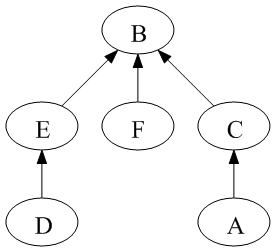
\includegraphics[height=3.5cm]{appendixds/appendixds-dsf-unionexample-after1.png}\hspace{2mm}}%
	%
	\hspace{4mm}%
	%
	\subfigure[Making B the child of C]
	{\hspace{6mm}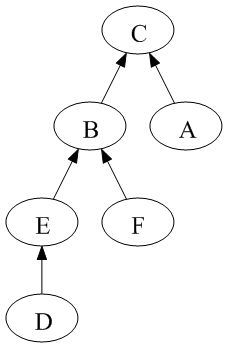
\includegraphics[height=4.8cm]{appendixds/appendixds-dsf-unionexample-after2.png}\hspace{6mm}}%
\caption{When unioning sets in a DSF, make the smaller tree's root the child of the larger tree's root to minimise the height of the result -- here, C should be made the child of B.}
\label{fig:appendixds-dsf-unionexample}
\end{stusubfig}
%---

\begin{enumerate}

\item Rather than arbitrarily choosing which tree root should be the child of the other, the \textbf{union-by-rank} approach aims to approximate the ideal that when a UNION takes place, the root of the tree representing the smaller subset becomes the child of the root of the tree representing the larger subset, and not the other way round. This is sensible, because the alternative leads to trees of greater height, making FIND-SET operations more costly. However, rather than maintaining the actual size of each subset, which would necessitate more work, union-by-rank works by giving each node a \emph{rank} (which is maintained as an upper bound on the height of the node from the bottom of its tree) and making the root with the smaller rank the child of the root with the larger rank.

\item It is better to have short paths from each node to the root of its tree, because it makes FIND-SET operations more efficient. The \textbf{path compression} approach takes advantage of the walking up the tree done during FIND-SET operations to set the parent links of visited nodes to point directly to the tree root. This makes future FIND-SET operations more efficient (see Figure~\ref{fig:appendixds-dsf-findsetexample}).

\end{enumerate}

%---
\begin{stusubfig}{p}
	\subfigure[The initial forest]
	{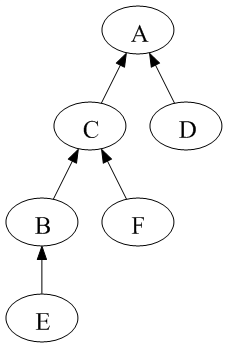
\includegraphics[height=4.8cm]{appendixds/appendixds-dsf-findsetexample-before.png}}%
	%
	\hspace{4mm}%
	%
	\subfigure[After FIND-SET(E)]
	{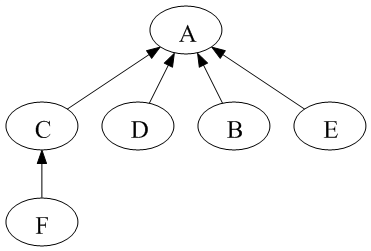
\includegraphics[height=3.5cm]{appendixds/appendixds-dsf-findsetexample-after.png}}%
\caption{Paths are compressed during FIND-SET calls -- here, future FIND-SET(B) and FIND-SET(E) calls will be constant time.}
\label{fig:appendixds-dsf-findsetexample}
\end{stusubfig}
%---

\noindent Bearing these optimizations in mind, the operations can then be implemented as shown in Listing~\ref{code:appendixds-dsf} (note that the names have been changed to match those in earlier listings, but the operations are exactly the same). The code itself is largely identical to the implementations originally given in \cite{worrell06}, but is slightly adapted to additionally support the storage of auxiliary data with each node. An example sequence of disjoint set operations is illustrated in Figure~\ref{fig:appendixds-dsf-example}.

%---
\begin{stulisting}[p]
\caption{Disjoint Set Forest Implementation}
\label{code:appendixds-dsf}
\lstinputlisting[style=Default]{appendixds/appendixds-dsf.lst}
\end{stulisting}
%---

%---
\begin{stusubfig}{p}
	\subfigure[The initial forest]
	{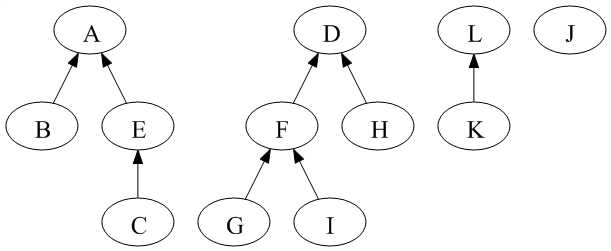
\includegraphics[width=.45\linewidth]{appendixds/appendixds-dsf-example-a.png}}%
	%
	\hspace{4mm}%
	%
	\subfigure[After UNION(G,K)]
	{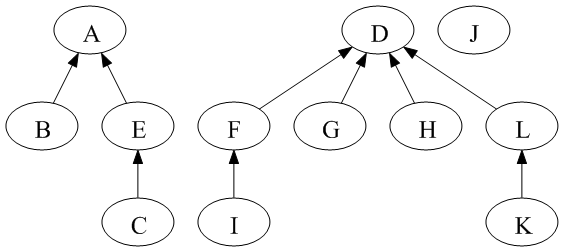
\includegraphics[width=.45\linewidth]{appendixds/appendixds-dsf-example-b.png}}%
	%
	\hspace{4mm}%
	%
	\subfigure[After UNION(J,B)]
	{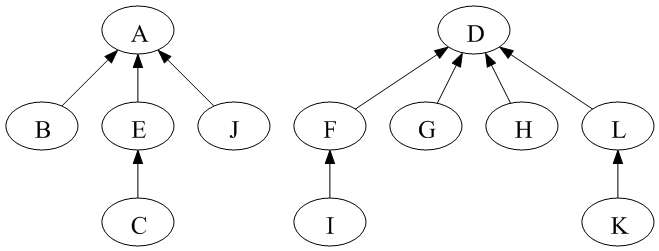
\includegraphics[width=.45\linewidth]{appendixds/appendixds-dsf-example-c.png}}%
	%
	\hspace{4mm}%
	%
	\subfigure[After FIND-SET(I)]
	{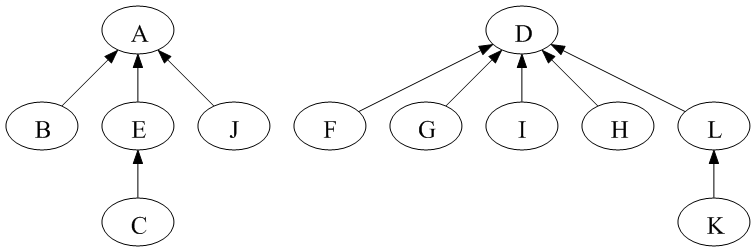
\includegraphics[width=.45\linewidth]{appendixds/appendixds-dsf-example-d.png}}%
\caption{An example DSF operation sequence -- note that some path compression happens even during UNION operations, since UNION calls FIND-SET internally.}
\label{fig:appendixds-dsf-example}
\end{stusubfig}
%---

\index{disjoint set forests|)}

\afterpage{\clearpage}
\newpage

%##################################################################################################
\section{Rooted Minimum Spanning Trees}
\label{sec:appendixds-rmsts}
%##################################################################################################

\index{rooted MSTs|(}

From basic graph theory, recall that given a positively-weighted, undirected graph $G = (V,E,w)$ with vertex set $V$, edge set $E$ and weight function $w: E \times E \to \mathbb{R}^+$, we say that $T$ is a (there can be more than one possibility) minimum spanning tree (MST) for $G$ iff:
%
\begin{enumerate}
\item $T$ is a \emph{tree}, i.e.~$T$ is a connected, acyclic graph.
\item $T$ \emph{spans} $G$, i.e.~$T$'s vertex set is also $V$.
\item $T$ is of \emph{minimum weight}, i.e.~there is no spanning tree of $G$ whose edge weights sum to a strictly lesser value than the edge weights of $T$.
\end{enumerate}
%
For our purposes here, we build on this definition to define a \emph{rooted MST}, which is just an MST with a defined root node (this is the type of MST used by the waterfall algorithms described in Chapter~\ref{chap:segmentation}). In implementation terms, this makes a significant difference, because we can then assign each vertex a parent and then traverse the tree in the usual recursive manner (with an unrooted tree, we have to treat the tree as a graph, which complicates the algorithms somewhat).

%################################################
\subsection{Construction}
%################################################

\index{rooted MSTs!construction|(}

%---
\begin{stulisting}[p]
\caption{Constructing a Rooted MST}
\label{code:appendixds-rootedmst-construction}
\lstinputlisting[style=Default]{appendixds/appendixds-rootedmst-construction.lst}
\end{stulisting}
%---

%---
\begin{stulisting}[p]
\caption{Merging Nodes in a Rooted MST}
\label{code:appendixds-rootedmst-mergenodes}
\lstinputlisting[style=Default]{appendixds/appendixds-rootedmst-mergenodes.lst}
\end{stulisting}
%---

\afterpage{\clearpage}

There are several algorithms for constructing normal MSTs of graphs, the best-known of which are perhaps Kruskal's algorithm (which sorts the edges in non-decreasing order of weight and then adds edges -- starting from the one with the smallest weight -- that do not create a cycle until all the vertices have been spanned) and Prim's algorithm (which maintains a set of spanned vertices -- initially an arbitrary start vertex -- and then repeatedly adds the smallest edge that connects a currently unspanned vertex to the vertices in this set until all the vertices have been spanned). To construct a \emph{rooted} MST, however, Prim's algorithm is superior to Kruskal's, because it works by gradually expanding a tree, starting from an initial vertex -- this can be easily adapted to build a rooted MST by choosing the initial vertex to be the root. A suitable implementation is shown in Listing~\ref{code:appendixds-rootedmst-construction}. This represents the tree using an adjacency graph (referred to using \texttt{base()} in the code) that stores parent pointers at each vertex. Constructing a rooted MST using Kruskal's algorithm would involve far more work, because Kruskal's adds edges all over the graph and only guarantees to join them up by the time the algorithm terminates.

\index{rooted MSTs!construction|)}

%################################################
\subsection{Node Merging}
%################################################

\index{rooted MSTs!node merging|(}

For rooted MSTs to be used as the underlying data structure for the various waterfall algorithms, they need to be augmented with a \emph{node merging} operation (see Listing~\ref{code:appendixds-rootedmst-mergenodes}). Since we're dealing with a rooted tree, the only nodes which can merge must form a parent/child pair in the tree. The basic algorithm is simple (remove one of the nodes and move its children across to the other one), but in practice things are slightly more complicated. The first step is to pick which node should survive and which should be removed. In the implementation here, the lower-indexed node is retained, because the rooted MSTs are being used in the construction of partition forests, which assign nodes an index corresponding to the lowest-indexed pixel they contain. Other implementations might want/need to make a different choice here.

The next step depends on whether we are retaining the parent of the pair being merged, or the child. If we are retaining the parent, we simply move all the child's children across to the parent (see Figures~\ref{fig:appendixds-mst-mergecases}(a) and (b)). If, on the other hand, we are retaining the child, we move all the parent's children \emph{except the child} across to the child (see Figures~\ref{fig:appendixds-mst-mergecases}(c) and (d)). Moving a node involves modifying its parent pointer to point to the surviving node and adding a graph edge that joins it to the surviving node (the graph edge joining it to the node being removed will be automatically removed when that node is).

%---
\begin{stusubfig}{p}
	\subfigure[Before merging to parent]
	{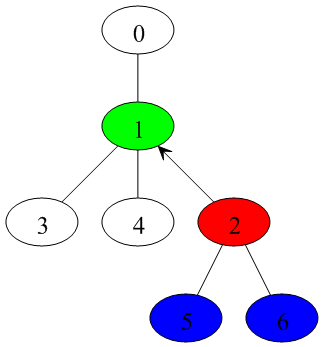
\includegraphics[height=5.5cm]{appendixds/appendixds-mst-mergetoparent-before.png}}%
	%
	\hspace{4mm}%
	%
	\subfigure[After merging to parent]
	{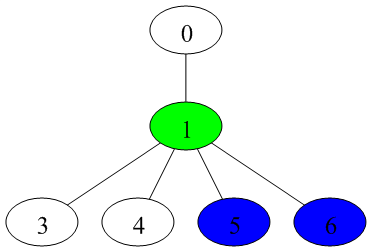
\includegraphics[height=4cm]{appendixds/appendixds-mst-mergetoparent-after.png}}%
	%
	\\
	%
	\subfigure[Before merging to child]
	{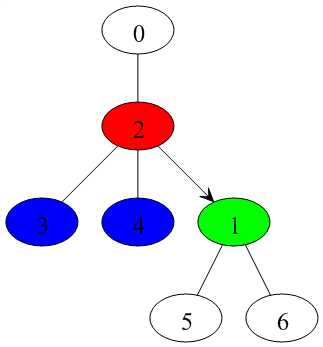
\includegraphics[height=5.5cm]{appendixds/appendixds-mst-mergetochild-before.png}}%
	%
	\hspace{4mm}%
	%
	\subfigure[After merging to child]
	{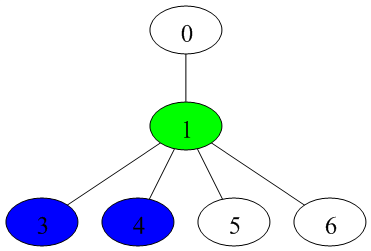
\includegraphics[height=4cm]{appendixds/appendixds-mst-mergetochild-after.png}}%
\caption{The two merging cases (see text for description) -- in each case, the green node is the surviving node, the red node is the one being removed and the blue nodes are the ones that are moved during the merging process.}
\label{fig:appendixds-mst-mergecases}
\end{stusubfig}
%---

It is important to check whether the root node is the one being removed -- if so, we need to make the surviving node into the new root node. Finally, we remove the node as planned and return the index of the surviving node.

\index{rooted MSTs!node merging|)}
\index{rooted MSTs|)}
